% Section 1-1
\section{电路和电路模型}

\subsection{电路}
由电阻器、电容器、线圈、变压器、晶体管、运算放大器、传输线、电池、发电机和信号发生器等
电器器件和设备连接而成的电路,称为实际电路。
根据实际电路的集合尺寸($d$)与其工作信号波长($\lambda$)的关系,可以将它们分为两大类:
满足 $d\ll\lambda$ 条件的电路称为集总参数电路,
其特点是电路中任意两个端点间的电压和流入任一器件端钮的电流是完全确定的,
与器件的几何尺寸和空间位置无关。不满足 $d\ll\lambda$ 条件的另一类电路称为分布参数电路。
本书只讨论集总参数电路,今后简称为电路。

\subsection{电路模型}
研究集总参数电路特性的一种方法是用电器仪表对实际电路直接进行测量。
更重要的一种方法是将实际电路抽象为电路模型,用电路理论的方法分析计算出电路的电气特性。
对于集总参数电路,当不关心器件内部的情况,只关心器件端钮上的电压和电流时,
可以定义一些理想化的电路元件来近似模拟器件端钮上的电气特性。
定义电阻元件是一种只吸收电能(可以转换为其他形式的能量)的元件,
电容元件是一种只存储电场能量的元件,
电感元件是一种只存储磁场能量的元件。
在电路分析中,为了便于看出电路模型中各元件的连接关系,
常采用仅仅表示元件连接关系的拓扑结构图。

图 \ref{fig:fig1_1_1} 列举了本书采用的部分电路元件的图形符号\footnote{由于时间紧迫,先拍照借图}。

\begin{figure}[htbp]
\centering
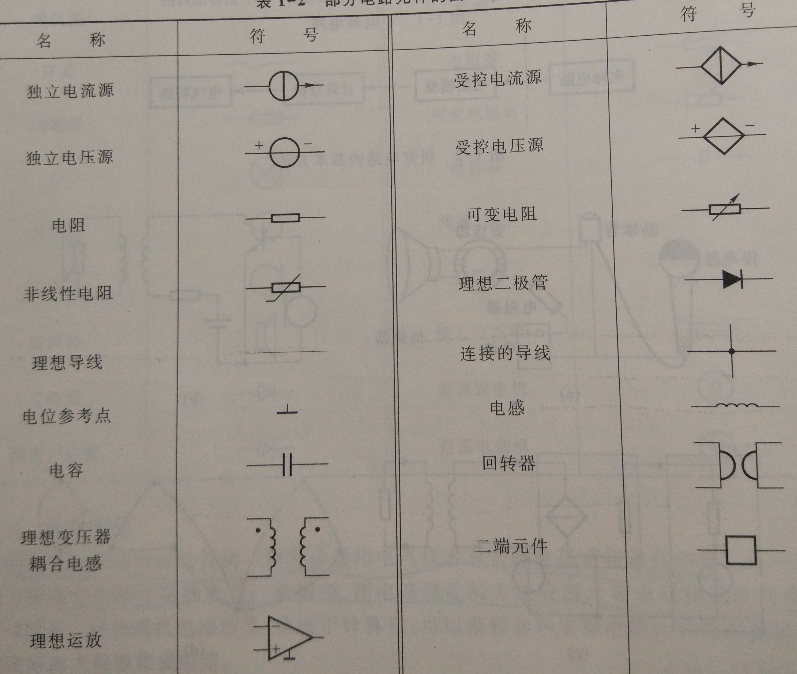
\includegraphics[scale=0.4]{s1-1-g.png}
\caption{部分电路元件的图形符号}\label{fig:fig1_1_1}
\end{figure}

电路模型近似地描述实际电路的电气特性。
根据实际电路的不同工作条件以及对模型精确度的不同要求,
应当用不同的电路模型模拟同一实际电路。

本课程的主要任务是研究电路模型(简称为电路)的各种分析方法,
其目的是通过对电路的分析研究来预测实际电路的电气特性,
以便指导改进实际电路的电气特性和设计制造出新的实际电路。
电路的研究问题可以分为两类。
一类是电路分析:已知电路结构和元件特性,分析电路的特性;
另一类是网络综合:根据电路特性的要求来设计电路的结构和元件参数。
本课程是电路的入门课程,主要讨论电路分析问题,也给出一些电路设计的例题。

今后,“电路”可能指实际电路,也可能指实际电路的电路模型。
